\documentclass{article}

\usepackage{graphicx}
\usepackage{subfigure}
\usepackage[hypcap]{caption}
\usepackage{listings}
\usepackage{float}
\floatstyle{plaintop}
\restylefloat{table}

\title{Experimental Design and Data Analysis: Assignment 2}
\author{Andrew Bedard \& Simone van Gompel(2567525) \\ Group 19}

\begin{document}

  \maketitle

  \section{Exercise 1}
  \subsection*{1}
  	Look at Fig:\ref{fig:Pairs} for the pairwise graph....
  	The variables that appear from inspection to correlate with migration are age and weight.

    \begin{figure}
      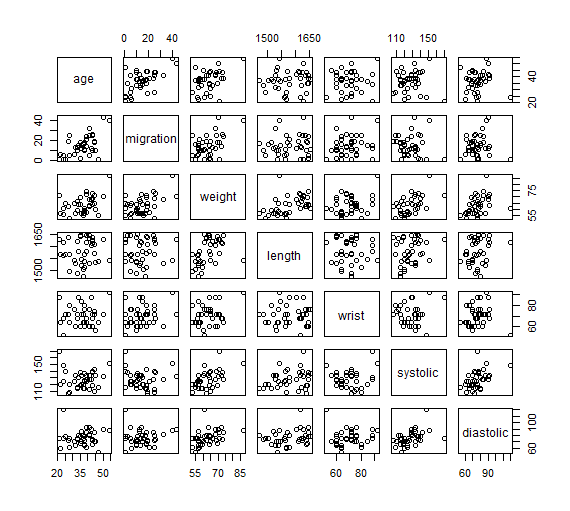
\includegraphics[scale=0.6]{../results/Pairs.png}
      \caption{Pairwise scatterplots of the dataset peruvians}
      \label{fig:Pairs}
    \end{figure}
    
    \subsection*{2}
    Using the Pearson (rank?) correlation test for all variables against migration we obtain the following results:
    \newline
    \centering
    \begin{tabular}{|c|c|c|c|c|c|c|c|}
    \hline 
     & age & migration & weight & length & wrist & systolic & diastolic \\ 
    \hline 
    migration & 0.58821250 & 1 & 0.48115337 & 0.07259415 & 0.23690464 & -0.08748046 & 0.07579214 \\ 
    \hline 
    \end{tabular} 
    
    Age was the most obviously correlated variable between migration 
\end{document}